\documentclass[11pt, oneside]{article}   	% use "amsart" instead of "article" for AMSLaTeX format
\usepackage{geometry}                		% See geometry.pdf to learn the layout options. There are lots.
\geometry{letterpaper}                   		% ... or a4paper or a5paper or ... 
%\geometry{landscape}                		% Activate for for rotated page geometry
%\usepackage[parfill]{parskip}    		% Activate to begin paragraphs with an empty line rather than an indent
\usepackage{graphicx}				% Use pdf, png, jpg, or eps� with pdflatex; use eps in DVI mode
								% TeX will automatically convert eps --> pdf in pdflatex		
\usepackage{amssymb}
\usepackage{amsmath}
\usepackage{parskip}
\usepackage{color}
\usepackage{hyperref}

\title{Limit of (1 + 1/n) to the nth power}
%\author{The Author}
%\section{}
%\subsection*{}
\date{}							% Activate to display a given date or no date

\graphicspath{{/Users/telliott_admin/Dropbox/Tex/png/}}
% \begin{center} 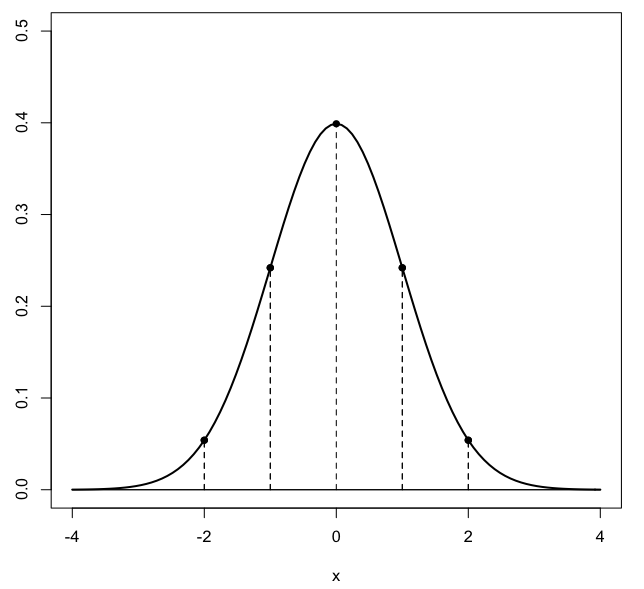
\includegraphics [scale=0.4] {gauss3.png} \end{center}
\begin{document}
\maketitle
\Large 
Our goal for this write-up is to find this limit:
\[ \lim_{n \rightarrow \infty} (1 + \frac{1}{n})^n \]
Massage it a bit
\[ (1 + \frac{1}{n})^n = e^{\ln \ [ \  (1 + 1/n)^n \ ] \ } \]
\[ = e^{n \ln (1 + 1/n)} \] 
so we want
\[ =  \lim_{n \rightarrow \infty} e^{n \ln (1 + 1/n)} \]
We will show that the limit of the exponent is equal to $1$:
\[ \lim_{n \rightarrow \infty} n \ln (1 + \frac{1}{n}) = 1 \]
Rearrange slightly
\[ =  \lim_{n \rightarrow \infty} \frac{\ln (1 + \frac{1}{n})}{1/n} \]
Note that the limit of both numerator and denominator is zero.  Therefore, we can apply L'Hopital's Rule.  If $f(n)$ is the numerator and $g(n)$ is the denominator
\[ \lim_{n \rightarrow \infty} \frac{f(n)}{g(n)} =  \lim_{n \rightarrow \infty} \frac{f'(n)}{g'(n)} \]
then by the chain rule
\[ f'(n) =  \frac{1}{1 + 1/n} \cdot (-n^{-2}) \]
Since $g'(n) = -n^{-2}$, we have just
\[ = \lim_{n \rightarrow \infty} \frac{1}{1 + 1/n} \]
which is indeed, just equal to $1$.  We have proved that
\[ \lim_{n \rightarrow \infty} (1 + \frac{1}{n})^n = e^1 = e \]
\subsection*{alternative}
Start by \emph{defining} a function that turns out to have all the properties of the logarithm (we've explored this approach elsewhere):
\[ L(x) = \int_1^x \frac{1}{t} \ dt \]
By standard properties of integrals:
\[ L(1) = \int_1^1 \frac{1}{t} \ dt = 0 \]
Define one more property, namely
\[ L(e) = \int_1^e \frac{1}{t} \ dt = 1 \]

Now, let $t$ be any number in the interval $[1,1+1/n]$.  We're interested in what happens as $n$ gets large.  This means that
\[ 1 \le t \le 1 + \frac{1}{n} \]
We will invert each term and rearrange as well:
\[ \frac{1}{1 + 1/n} \le \frac{1}{t} \le 1 \]
For each of these terms, we integrate $f(t) dt$ between $t = 1 \rightarrow 1 + 1/n$.  Remembering that $n$ is just a number and so is $1 + 1/n$ we have:
\[ \int_1^{1 + 1/n}  \frac{1}{1 + 1/n} \ dt \le  \int_1^{1 + 1/n} \frac{1}{t} \ dt \le \int_1^{1 + 1/n} 1 \ dt \]
The first term is 
\[ \int_1^{1 + 1/n}  \frac{1}{1 + 1/n} \ dt = \frac{1}{1 + 1/n} \cdot t  \ \bigg |_1^{1 + 1/n} \]
\[ =  \frac{1}{1 + 1/n} \cdot (1 + 1/n - 1) = \frac{1}{n+1} \]
The second term is
\[ \int_1^{1 + 1/n} \frac{1}{t} \ dt = L(1 + 1/n) \]
and the third is just $1/n$ so going back to the inequality we have established that
\[ \frac{1}{n+1} \le L(1 + 1/n) \le \frac{1}{n} \]
Exponentiate each term:
\[ e^{1/n+1} \le (1 + 1/n) \le e^{1/n} \]
Now, take the two inequalities separately.  We have
\[ e^{1/n+1} \le (1 + 1/n) \]
Raise to the power $n+1$
\[ e^{1} \le (1 + 1/n)^{n+1} \]
Divide by $1 + 1/n$ 
\[ = \frac{e}{1 + 1/n} \le (1 + 1/n)^{n} \]
Take the limit as $n \rightarrow \infty$ and we see that
\[  e \le \lim_{n \rightarrow \infty}  (1 + 1/n)^{n} \]
Similarly for the right-hand inequality:
\[ (1 + 1/n) \le e^{1/n} \]
Raise to the power $n$
\[ (1 + 1/n)^n \le e \]
So in the limit as $n \rightarrow \infty$ 
\[  \lim_{n \rightarrow \infty}  (1 + 1/n)^{n} \le e \]
And since
\[  e \le \lim_{n \rightarrow \infty}  (1 + 1/n)^{n} \le e \]
By the squeeze theorem, the middle term must be \emph{equal} to $e$
\[ \lim_{n \rightarrow \infty}  (1 + 1/n)^{n} = e \]

\end{document}